\chapter{Модули}
\label{modules}
\section{Что такое модули}
\label{what-are-modules}
\begin{wrapfigure}{l}{0.3\linewidth}
    
\includegraphics[width=1\linewidth]{modules.png}
\end{wrapfigure}

Работа с интерактивной оболочкой часто считается жизненно важной частью работы с динамическими языками программирования.
В ней удобно тестировать различный код и программы.
Чтобы использовать большую часть основных типов данных в Erlang, даже не нужно открывать текстовый редактор или сохранять файлы.
Можете отставить клавиатуру в сторону, сказать что на сегодня довольно, и пойти гулять.
Но если вы на этом остановитесь, то будете ужасным программистом на Erlang.
Чтобы использовать код, его нужно где\--то хранить!

Для этого и существуют модули.
Модуль \--- это несколько функций, сгруппированных в единый файл под одним именем.
Все функции в Erlang должны определяться в модулях.
Вы уже использовали модули, возможно даже не догадываясь об этом.
Встроенные функции \ops{hd} и \ops{tl}, которые упоминались в предыдущей главе, на самом деле входят в модуль \ops{erlang}, так же как и все арифметические, логические и булевы операторы.
ВФ из модуля \ops{erlang} отличаются от других функций тем, что при использовании Erlang они импортируются автоматически.
Вызов любой другой функции, определённой в модуле, должен выглядеть так: \ops{Module:Function(Arguments)}.

Смотрите:
\begin{lstlisting}[style=repl]
1> erlang:element(2, {a,b,c}).
b
2> element(2, {a,b,c}).
b
3> lists:seq(1,4).
[1,2,3,4]
4> seq(1,4).
** exception error: undefined shell command seq/2
\end{lstlisting}

В этом примере функция \ops{seq} из модуля list не была автоматически импортирована, тогда как \ops{element} была.
Ошибку ''undefined shell command'' генерирует оболочка, которая ищет и не находит команду оболочки (например, такую как \ops{f()}).
Некоторые функции из модуля \ops{erlang} не импортируются автоматически, но их используют не так часто.

Согласно логике, вы должны помещать функции, которые касаются похожих вещей, в один модуль.
Общие операции над списками хранятся в модуле \ops{lists}, а функции ввода\--вывода (которые позволяют выводить данные в консоль или файл), сгруппированы в модуле \ops{io}.
Единственный модуль, который не подчиняется этой схеме, это вышеупомянутый модуль \ops{erlang}, который содержит математические функции, функции преобразования, мультипроцессинга, изменения настроек виртуальной машины и т.д.
У этих функций нет ничего общего, кроме того, что все они считаются встроенными.
Лучше не создавать модули, похожие на \ops{erlang}, и сконцентрироваться на ясном логическом разделении функциональности.
\section{Объявление модуля}
\label{module-declaration}
\begin{wrapfigure}{l}{0.2\linewidth}
    
\includegraphics[width=1\linewidth]{declaration.png}
\end{wrapfigure}
При написании модуля можно объявлять два вида сущностей: функции и атрибуты.
Атрибуты это метаданные, которые описывают сам модуль: его имя, функции, которые должны быть видимы снаружи, автора кода и прочее.
Эти метаданные весьма полезны, так как подсказывают компилятору, как он должен производить обработку, а также позволяют людям извлекать из скомпилированного кода полезную информацию, не обращаясь к исходному коду.

В Erlang существует большое количество разнообразных атрибутов модулей.
Вы и сами можете объявить любые атрибуты на собственный вкус.
Но также существуют некоторые предопределённые атрибуты, которые будут появляться в вашем коде чаще других.
Все атрибуты модулей записываются в форме \ops{-Name(Attribute).}.
Чтобы ваш модуль можно было скомпилировать, необходим лишь один атрибут:

\begin{minipage}{1\linewidth}
    \textbf{-module(Name).}\\ 
    Этот атрибут всегда указывается первым оператором в файле и обозначает имя текущего модуля, где \emph{Name} это ~\ref{atoms}~атом.
    Это имя используется при вызове функций из другого модуля.
    Вызовы записывают в виде \ops{M:F(A)}, где \emph{M} это имя модуля, \emph{F} это имя функции и \emph{A} её аргументы.
\end{minipage}

Настало время немного попрограммировать!
Наш первый модуль будет простым и бесполезным.
Откройте текстовый редактор, введите указанную ниже строку, и сохраните под именем \ops{useless.erl}:
\begin{lstlisting}[style=repl]
-module(useless).
\end{lstlisting}

Всего лишь одна эта строка уже является рабочим модулем.
Конечно, без функций в нём нет никакого смысла.
Сначала давайте решим, какие функции будут экспортироваться из нашего <<бесполезного>> модуля.
Для этого нам понадобится ещё один атрибут:

\begin{minipage}{1.0\linewidth}
    \textbf{-export([Function1/Arity, Function2/Arity,\ldots,FunctionN/Arity]).}\\ 
    Он используется для определения функций модуля, которые можно вызывать извне.
    Атрибут содержит список функций с соответствующей им арностью.
    Арность функции это целое число, которые соответствует количеству аргументов, которые принимает функция.
    Это важная информация, поскольку разные функции, определённые в модуле, могут иметь одинаковое имя, только если их арность различается.
    Поэтому функции \ops{add(X, Y)} и \ops{add(X, Y, Z)} будут считаться различными и записываться в виде \ops{add/2} и \ops{add/3} соответственно.
\end{minipage}

\colorbox{lgray}{
    \begin{minipage}{1\linewidth}
        \textbf{Замечание:} экспортируемые функции представляют собой интерфейс модуля.
        Важно чтобы интерфейс сообщал о модуле только то, что необходимо для его использования и ничего более.
        Это позволяет менять скрытые детали вашей реализации, не нарушая работу кода, который может полагаться на ваш модуль.
    \end{minipage}
}

Сначала наш модуль экспортирует полезную функцию под названием <<add>>, которая принимает два аргумента.
Атрибут \ops{-export} можно добавить после объявления модуля:
\begin{lstlisting}[style=repl]
-export([add/2]).
\end{lstlisting}

Теперь напишем функцию:
\begin{lstlisting}[style=erlang]
add(A,B) ->
    A + B.
\end{lstlisting}

Синтаксис функции соответствует виду \ops{Name(Args) $->$ Body.}, где \emph{Name} должен быть атомом, а \emph{Body} это одно, либо несколько выражений Erlang, разделённых запятыми.
Функция должна заканчиваться точкой.
Обратите внимание, что Erlang не использует ключевое слово <<return>>.
От <<return>> никакой пользы!
Вместо этого автоматически будет возвращён результат выполнения последнего выражения в функции, и вам ничего для этого не нужно будет делать.

Добавьте следующую функцию (конечно же, какое руководство без <<Hello world>>!
Хоть даже и в четвёртой главе!), и не забудьте добавить её в атрибут \ops{-export}.
\begin{lstlisting}[style=erlang]
%% Shows greetings.
%% io:format/1 is the standard function used to output text.
hello() ->
io:format("Hello, world!~n").
\end{lstlisting}

Из этой функции нам станет понятно, что каждый комментарий должен начинаться с символа \ops{\%} и состоять из одной строки (то, что в примере используется \ops{\%\%}, не более чем вопрос стиля).
Также функция \ops{hello/0} демонстрирует как в вашем модуле можно вызывать функции из внешних модулей.
В данном случае это функция \ops{io:format/1}, которая является стандартной функцией для вывода текста (что объясняется в комментарии).

Добавим ещё одну функцию, которая будет использовать и \ops{add/2}, и \ops{hello/0}:
\begin{lstlisting}[style=erlang]
greet_and_add_two(X) ->
    hello(),
    add(X,2).
\end{lstlisting}
\begin{wrapfigure}[8]{l}{0.3\linewidth}
    
\includegraphics[width=1\linewidth]{imports.png}
\end{wrapfigure}

Не забудьте добавить\ops{greet\_and\_add\_two/1} в список экспортируемых функций.
Для вызовов \ops{hello/0} и \ops{add/2} указывать имя модуля не нужно, так как они были объявлены в текущем модуле.

Если бы вы захотели вызвать функцию \ops{io:format/1} так же как \ops{add/2} или любую другую функцию, определённую внутри модуля, то вам нужно было бы добавить в начале файла следующий атрибут: \ops{-import(io, [format/1]).}.
После этого можно сделать вызов \ops{format(''Hello, World!\~\strut n'').} напрямую.
Общий вид атрибута \ops{-import} подчиняется следующей формуле:
\begin{lstlisting}[style=erlang]
-import(Module, [Function1/Arity,..., FunctionN/Arity]).
\end{lstlisting}

Импорт функции это просто быстрый способ получить к ней доступ.
Программистам на Erlang не рекомендуется использовать атрибут \ops{-import}, так как считается, что это уменьшает читаемость кода.
К примеру, помимо функции \ops{io:format/2} существует также и функция \ops{io\_lib:format/2}.
Чтобы понять, какую из них использовал программист, придётся перейти в начало файла и посмотреть, из какого модуля функция была импортирована.
Поэтому использование имени модуля в качестве префикса считается хорошим стилем.
Обычно импортируют лишь функции, определённые в модуле lists, так как они используются намного чаще других.

Теперь ваш модуль \ops{useless} должен принять следующий вид:
\begin{lstlisting}[style=erlang]
-module(useless).
-export([add/2, hello/0, greet_and_add_two/1]).
 
add(A,B) ->
A + B.
 
%% Shows greetings.
%% io:format/1 is the standard function used to output text.
hello() ->
io:format("Hello, world!~n").
 
greet_and_add_two(X) ->
hello(),
add(X,2).
\end{lstlisting}

Мы закончили работать с нашим модулем <<useless>>.
Можете сохранить файл под именем \ops{useless.erl}.
Имя файла должно состоять из имени модуля, определённого в атрибуте \ops{-module}, и заканчиваться расширением '.erl', которое стандартно используется для файлов с исходным кодом Erlang.

Перед тем как скомпилировать модуль и, наконец\--то, опробовать его в деле, мы увидим как определять и использовать макросы.
В Erlang макросы очень похожи на выражения <<\#define>> в языке C, и, главным образом, используются для определения коротких функций и констант.
Они представляют собой простые текстовые выражения, которые будут заменены перед компиляцией кода.
Макросы полезны для того, чтобы не раскидывать по тексту ваших модулей <<магические>> значения.
Макрос определяется как атрибут модуля в виде \ops{-define(MACRO, some\_value).} и его можно использовать внутри модуля как \ops{?MACRO}.
Макрос в виде <<функции>> можно записать как \ops{-define(sub(X, Y), X - Y).} и использовать в виде \ops{?sub(23, 47)}.
Такой макрос позже будет заменён компилятором на выражение \ops{23 - 47}.
Кто\--то использует более сложные макросы, но общий синтаксис не меняется.
\section{Компилируем код}
\label{compiling-the-code}
Чтобы код Erlang мог использоваться виртуальной машиной, его компилируют в байт\--код.
Компилятор можно вызывать несколькими способами: из командной строки как \ops{\$ erlc flags file.erl}, из оболочки или в модуле как \ops{compile:file(FileName)}, в оболочке как \ops{c()} и т.д.

Пора скомпилировать наш бесполезный модуль и опробовать его.
Откройте оболочку Erlang и введите:
\begin{lstlisting}[style=erlang]
1> cd("/path/to/where/you/saved/the-module/").
"Path Name to the directory you are in"
ok
\end{lstlisting}

Оболочка будет искать по умолчанию файлы в той же директории, из которой она стартовала, а также в стандартной библиотеке.
Функция \ops{cd/1} определена только в оболочке Erlang.
Она позволяет изменить текущую директорию.
Пользователи Windows должны использовать в качестве разделителя директорий прямой слеш (косую черту \ops{\//}).
Когда мы поменяли текущую директорию на ту, в которой содержится наш модуль, вводим следующую команду:
\begin{lstlisting}[style=erlang]
2> c(useless).
{ok,useless}
\end{lstlisting}

Если сообщение, которое вы получили, отличается от приведённого выше, то убедитесь что файл назван правильно, что вы находитесь в правильной директории и в вашем модуле нет ошибок.
Когда компиляция пройдёт успешно, вы увидите, что в директории помимо \ops{useless.erl} появился ещё один файл \--- \ops{useless.beam}.
Это скомпилированный модуль.
Попробуем воспользоваться нашими функциями:
\begin{lstlisting}[style=erlang]
3> useless:add(7,2).
9
4> useless:hello().
Hello, world!
ok
5> useless:greet_and_add_two(-3).
Hello, world!
-1
6> useless:not_a_real_function().
** exception error: undefined function useless:not_a_real_function/0
\end{lstlisting}

Функции работают как и было задумано: \ops{add/2} складывает числа, \ops{hello/0} выводит <<Hello, world!>>, а \ops{greet\_and\_add\_two/1} делает и то и другое!
Вы, вероятно, задали себе вопрос: а почему функция \ops{hello/0} после вывода текста возвращает атом <<ok>>?
Потому что функции и выражения в Erlang \textbf{всегда} должны что\--то возвращать, даже когда в других языках они это делать не обязаны.
Поэтому функция \ops{io:format/1} возвращает <<ok>>, чтобы обозначить, что выполнение прошло нормально и ошибки отсутствуют.

В выражении 6 отображена ошибка, которая была сгенерирована из\--за отсутствия функции.
Если вы забыли проэкспортировать функцию, то получите сообщение именно такого типа.\\ 
\colorbox{lgray}
{
    \begin{minipage}{1\linewidth}
        \textbf{Замечание:} расширение '.beam', если вам интересно, означает \emph{Bogdan/Björn's Erlang Abstract Machine} (так называется виртуальная машина).
        Существуют также и другие виртуальные машины для Erlang, но сейчас они не более чем достояние истории, и их не используют.
        Среди них JAM (Joe's Abstract Machine, вобравшая черты Prolog WAM, и старая BEAM, которая предпринимала попытки компиляции из Erlang в C, и после \--- в нативный код.
        Измерения показали, что выигрыш от применения этого метода был слишком мал, поэтому от него отказались.
    \end{minipage}
}

Существует много флагов, которые позволяют тоньше контролировать процесс компиляции модуля.
Их список можно найти в \href{http://erlang.org/doc/man/compile.html}{документации Erlang}.
Вот наиболее востребованные флаги:\\ 

\begin{minipage}{0.9\linewidth}
    \textbf{-debug\_info}\\ 
    Добавляет в модуль отладочную информацию, которая необходима для работы инструментов Erlang, таких как отладчик, утилиты статического анализа и покрытия кода.
\end{minipage}

\begin{minipage}{0.9\linewidth}
    \textbf{-\{outdir,Dir\}}\\ 
    Компилятор Erlang будет по умолчанию создавать ''beam'' файлы в текущей директории.
    Этот флаг позволяет задать путь к директории, в которой будут сохраняться скомпилированные файлы.
\end{minipage}

\begin{minipage}{0.9\linewidth}
    \textbf{-export\_all}\\ 
    Флаг заставляет игнорировать атрибут модуля \ops{-export}.
    При этом будут проэкспортированы все функции, которые в нём определены.
    Главным образом этот флаг полезен при тестировании и разработке нового кода, и его не следует использовать на рабочих системах.
\end{minipage}

\begin{minipage}{0.9\linewidth}
    \textbf{\{d,Macro\} или \{d,Macro,Value\}}\\ 
    Определяет макрос, который можно будет использовать в модуле.
    \emph{Macro} должен быть атомом.
    Чаще всего этот флаг используется при юнит\--тестировании, чтобы гарантировать, что тестовые функции будут создаваться и экспортироваться только когда в них есть необходимость.
    По умолчанию элемент \emph{Value} имеет значение <<true>>, если не указан в списке явно.
\end{minipage}

Чтобы скомпилировать наш модуль \ops{useless} с использованием флагов, нужно выполнить одну из следующих директив:
\begin{lstlisting}[style=erlang]
7> compile:file(useless, [debug_info, export_all]).
{ok,useless}
8> c(useless, [debug_info, export_all]).
{ok,useless}
\end{lstlisting}

Также можно схитрить и определить флаги компиляции при помощи атрибутов прямо в самом модуле.
Чтобы получить такой же результат как в выражениях 7 и 8, необходимо добавить в модуль следующую строку: 
\begin{lstlisting}[style=erlang]
-compile([debug_info, export_all]).
\end{lstlisting}

Далее необходимо лишь скомпилировать модуль, и вы получите тот же результат, что и с флагами переданными вручную.
А теперь, когда мы можем записывать функции, компилировать их и исполнять, настало время узнать, что же мы сможем со всем этим сделать!\\ 
\colorbox{lgray}
{
    \begin{minipage}{1\linewidth}
        \textbf{Замечание:} модуль также можно скомпилировать в нативный код.
        Компиляция в нативный код доступна не для каждой платформы и ОС.
        Для платформ, которые допускают такую компиляцию, можно добиться ускорения программ (по неточным данным приблизительно на 20\%).
        Для компиляции в нативный код необходимо использовать модуль \ops{hipe}. Компиляция осуществляется при помощи команды: \ops{hipe:c(Module,OptionsList).}
        Также в оболочке можно использовать команду \ops{c(Module,[\{hipe,o3\}]).}
        Обратите внимание, что .beam файл, полученный в результате такой компиляции, нельзя переносить между платформами, тогда как обычные файлы можно.
    \end{minipage}
}
\section{Подробнее о модулях}
\label{more-about-modules}
Прежде чем переходить к написанию функций и кода, польза которых сомнительна, необходимо упомянуть ещё несколько фактов, которые в будущем могут пригодиться.

Первый из них касается метаданных в модулях.
Я упомянул в начале главы, что атрибуты модуля \---это метаданные, которые описывают сам модуль.
Как мы можем получить доступ к этим метаданным, если у нас нет доступа к исходному коду модуля?
В этом нам поможет компилятор.
При компиляции он соберёт атрибуты и сохранит их (вместе с другой информацией) в функции \ops{module\_info/0}.
Вот так будут выглядеть метаданные модуля \ops{useless}:
\begin{lstlisting}[style=erlang]
9> useless:module_info().
[{exports,[{add,2},
            {hello,0},
            {greet_and_add_two,1},
            {module_info,0},
    {module_info,1}]},
    {imports,[]},
    {attributes,[{vsn,[174839656007867314473085021121413256129]}]},
    {compile,[{options,[]},
            {version,"4.6.2"},
            {time,{2009,9,9,22,15,50}},
{source,"/home/ferd/learn-you-some-erlang/useless.erl"}]}]
10> useless:module_info(attributes).
[{vsn,[174839656007867314473085021121413256129]}]
\end{lstlisting}

Также в вышеприведённом тексте есть упоминание дополнительной функции \ops{module\_info/1}, которая позволит получить каждый элемент метаданных по отдельности.
В метаданных содержатся экспортируемые функции, импортируемые функции (в данном случае ни одной), атрибуты (в них можно хранить метаданные, которые определены вами), информация о компиляции и ключи компиляции.
Если бы вы решили добавить в модуль атрибут \ops{-author(``An Erlang Champ'').}, он оказался бы в том же разделе, где и \ops{vsn}.
Когда дело доходит до рабочей системы, для атрибутов модулей маловато применений, но они могут быть полезны для реализации маленьких хитростей: я использую их в \href{http://learnyousomeerlang.com/static/erlang/tester.erl}{тестовом скрипте}, чтобы описывать функции, для которых юнит\--тесты оставляют желать лучшего.
Скрипт сканирует атрибуты модуля, находит функции, снабжённые комментариями, и выдаёт о них предупреждения.\\ 
\colorbox{lgray}
{
    \begin{minipage}{1\linewidth}
        \textbf{Замечание:} \ops{vsn} это уникальное значение, которое генерируется автоматически и отличается для каждой версии вашего кода, исключая комментарии.
        Это значение используется при горячей загрузке кода (обновление приложения во время исполнения, без необходимости его остановки), а также некоторыми инструментами, которые связаны с управлением релизами.
        Если хотите, можете сами указать значение для \ops{vsn}: просто добавьте в модуль атрибут \ops{-vsn(VersionNumber)}.
    \end{minipage}
}

\begin{wrapfigure}{r}{0.4\linewidth}
    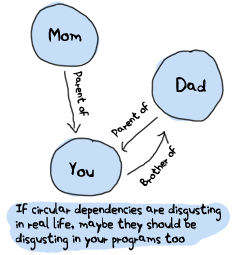
\includegraphics[width=1\linewidth]{circular-dependencies.png}
\end{wrapfigure}
Ещё один момент, на который стоит обратить внимание при проектировании модулей: избегайте циклических зависимостей!
Модуль \emph{A} не должен вызывать модуль \emph{B}, который в свою очередь вызывает модуль \emph{A}.
Такие зависимости приводят к усложнению поддержки кода.
Кому хочется проснуться посреди ночи от того, что маньяк\--разработчик пытается выдавить вам глаза из\--за чудовищного кода, который вы написали.

По той же причине (поддержка кода и забота о вашим зрении), обычно считается хорошим тоном размещение рядом функций близких по назначению.
В качестве примера можно привести функции запуска и остановки приложения, или создания и удаления записи в некоторой базе данных.

Ну что ж, довольно нравоучений.
Готовы узнать ещё немного об Erlang?
